\chapter{Standard IEEE/ETSI}

In questo capitolo, viene presentata un'introduzione teorica approfondita agli standard e alle tecnologie che hanno guidato le nostre scelte progettuali e di ciò che riveste maggiore importanza. La comprensione di questi standard è essenziale per contestualizzare le scelte fatte e per apprezzare i risultati riscontrati. Ci si concentrerà su diversi protocolli e specifiche tecniche che hanno influenzato lo sviluppo del testbed scelto, esplorando le loro caratteristiche distintive, le modalità di funzionamento e le varie applicazioni pratiche.

In particolare, si inizierà con un'analisi qualitativa dello standard IEEE 802.11, che rappresenta la base delle comunicazioni wireless. Questo standard ha introdotto una serie di tecnologie e protocolli fondamentali per la gestione delle reti senza fili, costruendo le basi per applicazioni avanzate, inclusi i sistemi automotive.

Successivamente, ci si focalizzerà su \textit{WAVE (Wireless Access in Vehicular Environments)}, un protocollo cruciale per la connettività dei veicoli e la gestione delle reti di trasporto intelligenti (ITS). WAVE consente la comunicazione tra singoli veicoli e tra veicoli ed infrastrutture, facilitando la trasmissione di informazioni vitali per la sicurezza e l'efficienza del traffico automobilistico.

Un altro aspetto chiave che verrà trattato è il meccanismo \textit{EDCA (Enhanced Distributed Channel Access)}, che rappresenta un'evoluzione del livello \textit{MAC (Media Access Control)} nelle reti wireless. EDCA introduce un metodo di accesso al canale più sofisticato rispetto al tradizionale \textit{DCF (Distributed Coordination Function)}, consentendo una gestione più efficiente delle priorità di traffico. Questo è particolarmente rilevante in scenari in cui coesistono diversi tipi di traffico (e.g. video, voce e dati) ognuno con requisiti specifici di latenza e larghezza di banda. Verrà discusso come EDCA assegni diverse code di accesso per garantire che le comunicazioni più critiche ricevano la priorità necessaria, migliorando così l'esperienza complessiva degli utenti.

Verrà, successivamente, esaminato lo standard \textit{ETSI DCC (Dedicated Short Range Communications)}, che si integra con le tecnologie precedentemente menzionate per supportare comunicazioni a corto raggio e per applicazioni specifiche nel settore automotive. DCC è progettato per garantire comunicazioni affidabili e tempestive tra veicoli e tra veicoli e infrastrutture, contribuendo a una mobilità più sicura ed efficiente.

Per concludere, verrà delineato lo standard ETSI ITS-G5, illustrando le caratteristiche che lo accomunano con le controparti di IEEE e quelle che lo differenziano

\section{IEEE 802.11}
Viene fatto un excursus molto breve sull'IEEE 802.11, che servirà come introduzione agli argomenti successivi. L'IEEE 802.11 è un insieme di standard e successivi emendamenti sviluppati dall'Institute of Electrical and Electronics Engineers (IEEE) per le comunicazioni wireless, comunemente conosciuto come Wi-Fi. Questi standard definiscono le specifiche per la trasmissione di dati in reti locali senza fili, coprendo vari aspetti come il livello fisico (PHY) e il controllo dell'accesso al mezzo (MAC) \cite{ieee80211}.

E' ormai all'ordine del giorno che l'adozione dell'IEEE 802.11 ha rivoluzionato il modo in cui ci si connette a Internet e si scambiano le informazione, rendendo possibile l'accesso wireless ad una vasta gamma di dispositivi, dai computer portatili agli smartphone. Gli standard 802.11 sono stati aggiornati nel corso degli anni per migliorare la velocità, la sicurezza e l'affidabilità delle comunicazioni.

Nel contesto delle comunicazioni \textit{C-ITS (Cooperative Intelligent Transport Systems)}, l'IEEE 802.11 è particolarmente rilevante poiché la sua architettura e le sue tecniche di accesso al canale sono state adottate nell'architettura ITS-G5 \cite{etsi302} e, quindi, comprendere le sue basi è essenziale per apprezzare come queste tecnologie possano essere integrate per supportare la comunicazione tra veicoli e infrastrutture, migliorando la sicurezza stradale e l'efficienza del traffico.

\subsection[Caratteristiche]{Caratteristiche}
L'IEEE 802.11 è un insieme di standard sviluppato dall'Institute of Electrical and Electronics Engineers (IEEE) per la comunicazione wireless nelle reti locali (WLAN), comunemente conosciuto come Wi-Fi. Questi standard definiscono le specifiche per la trasmissione di dati su reti senza fili e hanno subito diverse evoluzioni nel corso degli anni.

La prima versione, 802.11-1997, offriva una velocità massima di 2 Mbps e operava nella banda di frequenza a 2.4 GHz. Nel 1999, sono stati introdotti gli standard 802.11b e 802.11a. L'802.11b ha aumentato la velocità massima a 11 Mbps, diventando il primo standard Wi-Fi ampiamente adottato, mentre l'802.11a operava a 5 GHz e supportava velocità fino a 54 Mbps, sebbene avesse una portata inferiore rispetto all'802.11b. Successivamente, nel 2003, è stato introdotto l'802.11g, che combinava le migliori caratteristiche dei due standard precedenti, supportando velocità fino a 54 Mbps nella banda a 2.4 GHz.

L'802.11n, lanciato nel 2009, ha introdotto la tecnologia MIMO (Multiple Input Multiple Output), aumentando la velocità fino a 600 Mbps e migliorando l'efficienza della rete \cite{evolution}. Nel 2013, l'802.11ac ha operato principalmente a 5 GHz, supportando velocità superiori a 1 Gbps grazie a tecnologie avanzate come il beamforming. Infine, l'802.11ax, noto anche come Wi-Fi 6, è stato introdotto nel 2019, apportando miglioramenti significativi in termini di efficienza, capacità e prestazioni in ambienti affollati, con velocità teoriche che possono raggiungere fino a 9.6 Gbps. È previsto che l'802.11be, o Wi-Fi 7, sarà disponibile nel 2024, introducendo ulteriori miglioramenti in termini di velocità e latenza (Figura \ref{fig:evo}).

\begin{figure}[h!]
    \centering
    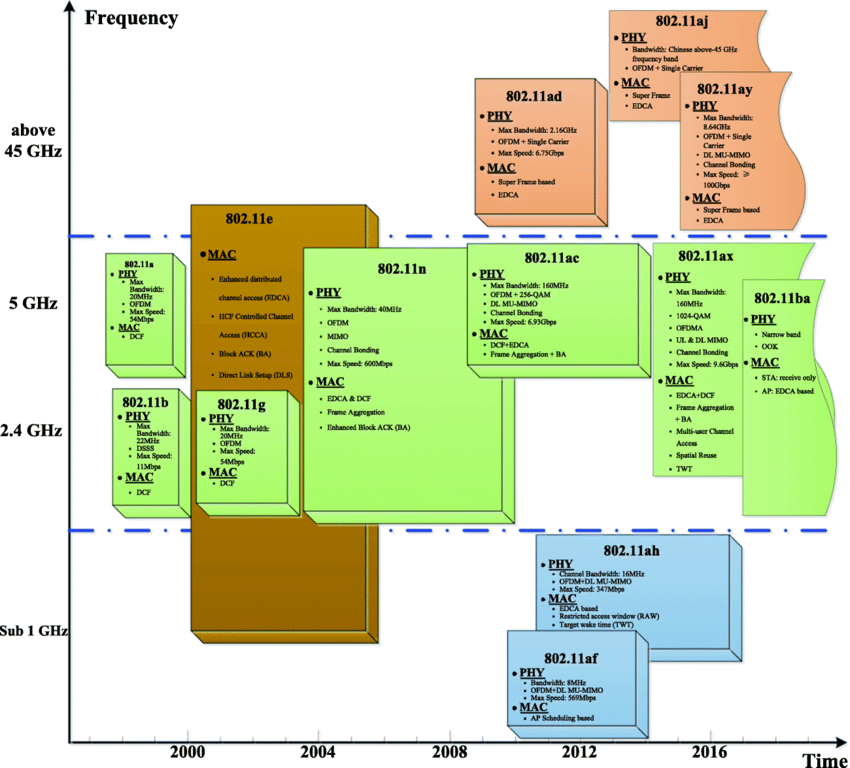
\includegraphics[width=1\textwidth]{evolution.png}
    \caption{Evoluzione dello standard IEEE 802.11}
    \label{fig:evo}
\end{figure}

Un aspetto fondamentale del protocollo IEEE 802.11 è la Distributed Coordination Function (DCF), che rappresenta il metodo standard per l'accesso al canale di comunicazione. DCF è simile al protocollo CSMA/CA (\textit{Carrier Sense Multiple Access with Collision Avoidance}) utilizzato nelle reti cablate quali Ethernet et simila; verrà descritto successivamente.

Non meno importante è l'emendamento IEEE 802.11p (IEEE WAVE), che sarà descritto in modo approfondito successivamente. Questo standard è particolarmente rilevante per le applicazioni di comunicazione veicolare e per la gestione della sicurezza nelle reti di trasporto.

Le caratteristiche tecniche degli standard 802.11 includono l'operatività nelle bande di frequenza a 2.4 GHz e 5 GHz, con l'802.11ax che introduce anche la banda a 6 GHz. Questi standard utilizzano diverse tecniche di modulazione, come BPSK, QPSK e 16-QAM, per ottimizzare la trasmissione dei dati. La larghezza di banda varia: mentre gli standard precedenti utilizzavano larghezze di banda di 20 MHz e 40 MHz, gli standard più recenti come 802.11ac e 802.11ax possono utilizzare larghezze di banda fino a 160 MHz. La tecnologia MIMO consente l'uso di più antenne per trasmettere e ricevere dati simultaneamente, migliorando la capacità e la velocità della rete, mentre il beamforming ottimizza la direzione del segnale verso il dispositivo ricevente, migliorando la portata e l'affidabilità della connessione.

Per quanto riguarda la sicurezza, gli standard 802.11 hanno evoluto i protocolli di protezione nel tempo. Il primo protocollo, WEP (Wired Equivalent Privacy), si è rivelato vulnerabile a vari attacchi, portando all'introduzione di WPA (Wi-Fi Protected Access), che offriva una maggiore sicurezza. Successivamente, WPA2, basato su AES (Advanced Encryption Standard), ha fornito una protezione robusta, mentre WPA3, l'ultima evoluzione, migliora ulteriormente la sicurezza, specialmente in ambienti pubblici e per dispositivi IoT.

\subsection[DCF]{Distributed Coordination Function}
La Distributed Coordination Function (DCF) è la modalità standard attraverso cui i dispositivi Wi-Fi accedono al canale di comunicazione, simile al protocollo CSMA/CA (\textit{Carrier-sense multiple access with collision avoidance}) utilizzato nelle reti cablate, tipo Ethernet et simila. Quando un nodo inizia a trasmettere dati, gli altri dispositivi devono attendere che il canale diventi libero prima di poter inviare le proprie informazioni (\textit{Carrier-sense}).

Dopo che una stazione ha completato la trasmissione dei dati, c'è un intervallo chiamato Short Interframe Space (SIFS), durante il quale l'access point (AP) attende prima di inviare un pacchetto di conferma (ACK). Una volta ricevuto l'ACK, la seconda stazione deve attendere il Distributed Interframe Space (DIFS), che è un periodo di tempo definito per consentire a più nodi di accedere al canale (\textit{Collision Avoidance} - Figura \ref{fig:dcf}). È fondamentale che SIFS sia minore di DIFS, poiché ciò consente ai nodi di tentare di trasmettere i dati, sebbene non necessariamente di farlo immediatamente.

\begin{figure}[h!]
    \centering
    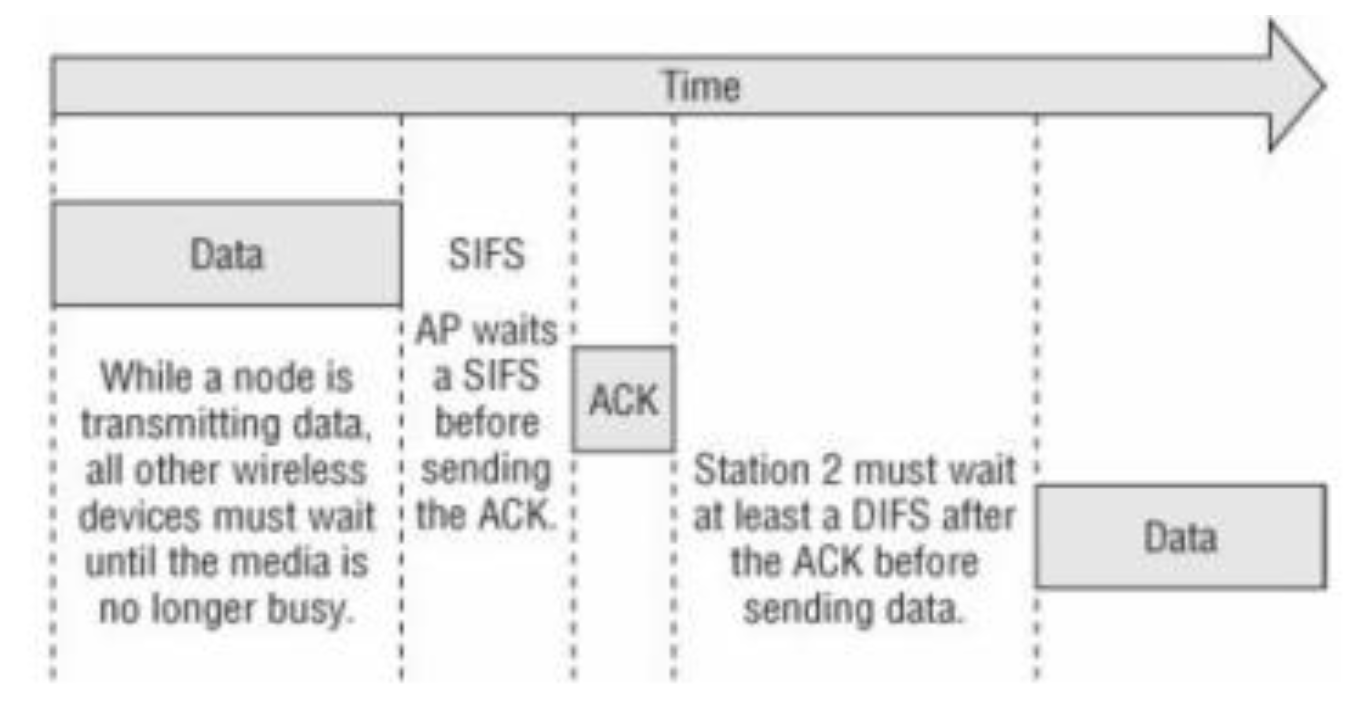
\includegraphics[width=0.7\textwidth]{dcf.png}
    \caption{Distributed Coordination Function}
    \label{fig:dcf}
\end{figure}

Se il canale risulta ancora occupato, il nodo non può semplicemente attendere il DIFS; deve considerare un ulteriore intervallo di backoff per evitare conflitti. Il backoff è un valore casuale scelto all'interno di un intervallo definito da [0, CW], dove CW rappresenta la congestion window, e il suo valore può variare a seconda della situazione della rete. Minore è il valore di CW, minore sarà l'intervallo di attesa. Durante il periodo di contesa, il canale rimarrà inattivo per uno slot temporale, consentendo di decrementare il valore di CW e ridurre l'intervallo di attesa, specialmente in caso di congestione.

Sebbene DCF sia un meccanismo efficace per la condivisione del canale tra più stazioni, presenta alcune limitazioni significative. Innanzitutto, non esiste un controllo della congestione, il che può portare a collisioni. Le collisioni multiple possono limitare la banda disponibile e causare seri problemi di trasmissione. Inoltre, DCF non garantisce alcuna Quality of Service (QoS), non essendoci un metodo per prioritizzare i flussi di traffico.

Per affrontare queste problematiche, esiste un'altra soluzione chiamata Point Coordination Function (PCF), che può essere utilizzata solo in configurazioni infrastrutturate, dove la connessione è gestita da un access point e include meccanismi per garantire la QoS. Tuttavia, poiché PCF non è adatta per il protocollo 802.11p, è necessario integrare la QoS direttamente nella Coordination Function (CF) per garantire prestazioni adeguate nelle reti che non possono utilizzare PCF. Tale problema è stato affrontato con lo sviluppo della EDCA con la \textit{EDCF (Enhanced Distributed Coordination Function)}, affrontata nella \autoref{edca}.

\section{IEEE WAVE}
\label{wave}
WAVE è progettato specificamente per ambienti di trasporto, consentendo la comunicazione tra veicoli (\textit{V2V: Vehicle-to-Vehicle}) e tra veicoli e infrastrutture stradali (\textit{V2I: Vehicle-to-Infrastructure}). Questo protocollo sfrutta canali wireless dedicati per garantire una bassa latenza e una maggiore affidabilità, elementi essenziali per applicazioni critiche come la prevenzione degli incidenti e la gestione del traffico. 

Per facilitare questo, l'IEEE ha introdotto un emendamento specifico al protocollo 802.11, noto come 802.11p \cite{std2007wireless}. Questo emendamento si occupa sia del livello fisico, chiamato PHY, sia della gestione dell'accesso al canale, che riguarda il livello MAC. Non ci si soffermerà ulteriormente sui livelli superiori, se non attraverso un breve excursus, poiché il protocollo in questione supporta senza difficoltà qualsiasi tipo di livello, sia esso basato su IP o meno \cite{DSRC-Based-vehicular}. E' importante sottolineare che è stato previsto un apposito protocollo per l'invio di frame che non richiedono un livello di trasporto come TCP o UDP, denominato \textit{WAVE Short Message Protocol (WSMP)}.

\begin{figure}[h!]
    \centering
    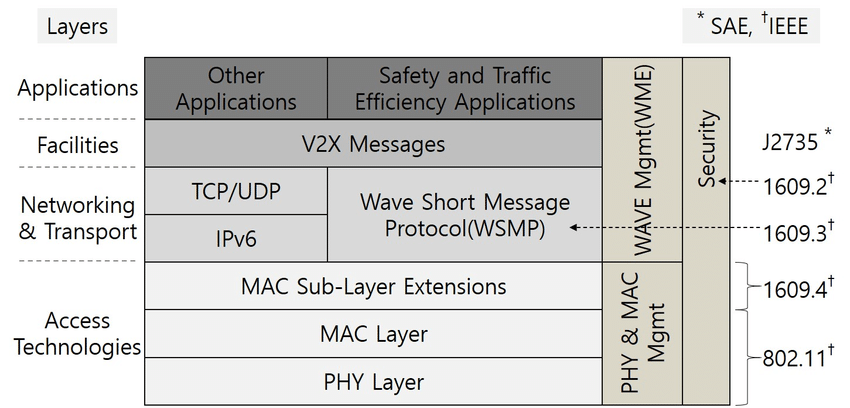
\includegraphics[width=0.7\textwidth]{WAVE-protocol-stack.png}
    \caption{Stack protocollo WAVE}
    \label{fig:wave_stack}
\end{figure}

Di seguito, viene presentato un elenco che fornisce ulteriori dettagli sui protocolli menzionati nella Figura \ref{fig:wave_stack}, partendo dal layer fisico e salendo di volta in volta:

\begin{itemize}
    \item \textit{IEEE 802.11-2016, IEEE Std 802.11p: Wireless Access in Vehicular Environments}.
    \item \textit{IEEE 1609.0: IEEE Guide for Wireless Access in Vehicular Environments (WAVE) Architecture}, con le sue varie  \cite{8686445}: 
        \begin{itemize}
            \item \textit{IEEE 1609.4: IEEE Standard for Wireless Access in Vehicular Environments (WAVE) - Multi-Channel Operation}; per il \textit{channel routing} e il \textit{channel coordination} \cite{7435228}.
            \item \textit{IEEE 1609.3: IEEE Standard for Wireless Access in Vehicular Environments (WAVE) - Networking Services}; per i sopracitati \textit{WAVE Short Messages} \cite{9374154}.
            \item \textit{IEEE 1609.2: IEEE Standard for Wireless Access in Vehicular Environments - Security Services for Applications and Management Messages}; per tutti gli aspetti relativi alla sicurezza \cite{10075082}.
        \end{itemize}
\end{itemize}

Risultano, anche, essere presenti altre varie componenti del protocollo \textit{IEEE 1609.0} su cui non ci si soffermerà e si riportano per completezza:

\begin{itemize}
    \item \textit{IEEE 1609.11:  IEEE Standard for Wireless Access in Vehicular Environments (WAVE) - Over-the-Air Electronic Payment Data}; standard per i pagamenti elettronici in applicazione \textit{WAVE based} \cite{5692959}.
    \item \textit{IEEE 1609.12:  IEEE Standard for Wireless Access in Vehicular Environments (WAVE) - Identifier Allocations}; standard per l'allocazione degli identificatori \textit{WAVE} \cite{8877516}.
\end{itemize}

Per concludere, alla luce del fatto che il contesto preso in esame, quello veicolare, richiede uno scambio di informazioni con latenze minime, \textit{WAVE} si basa interamente su una nuova modalità Wireless, simile alla classica \textit{ad hoc}, chiamata \textit{OCB (Outside Context of a Basic Service Set)}. Questo è un approccio che consente la trasmissione di dati al di fuori delle limitazioni tradizionali delle reti Wi-Fi, permettendo una comunicazione più flessibile e diretta tra i dispositivi, senza la necessità di passare attraverso infrastrutture quali i punti di accesso (\textit{Access Point}).

\subsection[Layer fisico]{Layer fisico}
L'IEEE 802.11p è uno standard della famiglia IEEE 802.11 progettato specificamente per la comunicazione wireless in ambienti vehicolari. È una tecnologia di rete che consente la comunicazione tra veicoli e tra veicoli e infrastrutture, facilitando applicazioni come la sicurezza stradale, la gestione del traffico e i servizi di infotainment.

Esso, innanzitutto, è basato su una modulazione OFDM (\textit{Orthogonal Frequencies Division Multiplexing}), ove in un totale di 64 sottoportanti, ne vengono utilizzate solo 52: 48 per la trasmissione delle informazioni e 4 di tipo pilota (Figura \ref{fig:ofdm}); supporta velocità differenti in base alla modulazione delle sottoportanti e alla larghezza di banda utilizzati.

\begin{figure}[h!]
    \centering
    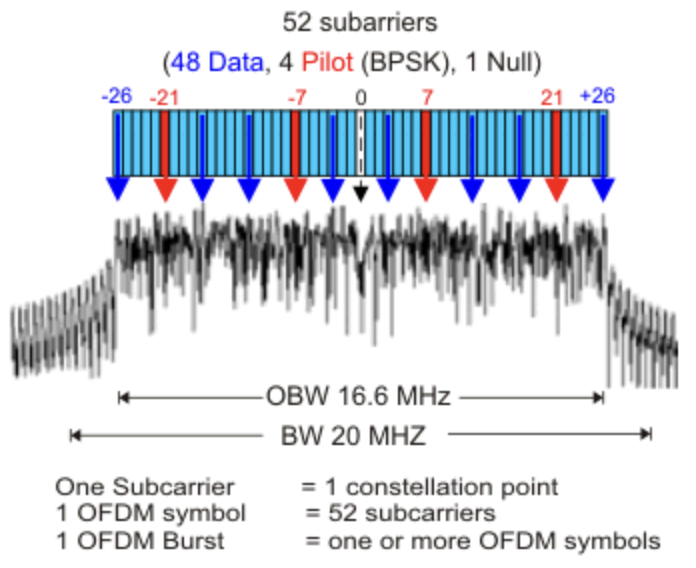
\includegraphics[width=0.4\textwidth]{ofdm.png}
    \caption{OFDM 802.11}
    \label{fig:ofdm}
\end{figure}

Di seguito una tabella riassuntiva dei parametri appena citati, suddivisi per \textit{bandwidth}:

%\clearpage % Forza la stampa delle tabelle e figure in sospeso

\begin{table}[htbp]
    \centering
    \begin{tabular}{|p{7em}|p{7em}|p{7em}|p{7em}|} 
     \hline
     \textbf{Parametri} & \textbf{20 MHz} & \textbf{10 MHz} & \textbf{5 MHz} \\ 
     \hline
     \textbf{Bit rate (Mbit/s)} & 6, 9, 12, 18, 24, 36, 48, 54 & 3, 4.5, 6, 9, 12, 18, 24, 27 & 1.5, 2.25, 3, 4.5, 6, 9, 12, 13.5 \\ 
     \hline
     \textbf{Modulation} & BPSK, QPSK, 16/64QAM & BPSK, QPSK, 16/64QAM & BPSK, QPSK, 16/64QAM \\
     \hline
     \textbf{Code rate} & 1/2, 2/3, 3/4 & 1/2, 2/3, 3/4 & 1/2, 2/3, 3/4 \\
     \hline
     \textbf{Subcarriers} & 52 & 52 & 52 \\
     \hline
     \textbf{Spacing} & 312.5 kHz & 156.25 kHz & 78.125 kHz \\ 
     \hline
    \end{tabular}
    \caption{Parametri delle diverse larghezze di banda}
    \label{table:1}
\end{table}

Parlando circa le frequenze utilizzate, l'IEEE 802.11p opera nella banda di frequenza di 5,9 GHz (5,850 - 5,925 GHz), con le larghezze di canale citate nella Tabella \ref{table:1}. Questo standard consente l'uso di circa 9 canali, come illustrato nella Figura \ref{fig:frequency}. Tra questi, i canali 172 (5.860 GHz) e 184 (5.920 GHz) sono dedicati alla sicurezza: il primo fornisce una soluzione robusta per la sicurezza, mentre il secondo funge da protezione contro la congestione su altri canali \cite{ad_hoc_new}.

\begin{figure}[h!]
    \centering
    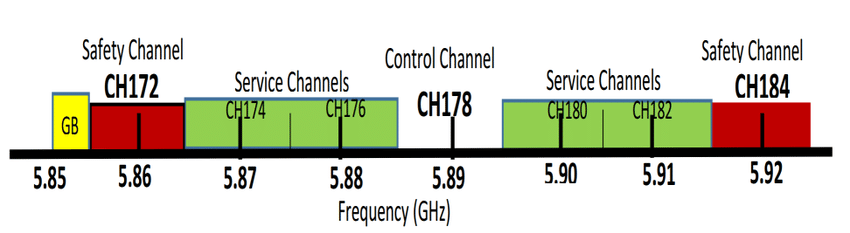
\includegraphics[width=0.7\textwidth]{frequency.png}
    \caption{Frequenze dell'IEEE 802.11p}
    \label{fig:frequency}
\end{figure}

Il canale 178 (5.890 GHz) è un canale di controllo, responsabile della gestione della trasmissione e della creazione del collegamento. Inoltre, sono disponibili sei canali di servizio per la comunicazione bidirezionale tra diversi tipi di unità.

\subsection[Layer MAC]{Layer MAC}
Non esiste una netta distinzione tra il layer MAC dell'IEEE 802.11p con il relativo omonimo del classico IEEE 802.11, se non per alcuni concetti:

\begin{itemize}
    \item come già esplicitato quando si è iniziato a parlare di \textit{WAVE} poc'anzi, esso si basa principalmente sulla modalità \textit{OCB} anzichè le classiche, come ad esempio la \textit{Infrastructure mode}.
    \item per l'accesso al canale, sfrutta una variante della \textit{DCF (Distributed Coordination Function)} chiamata \textit{EDCA (Enhanced Distributed Channel Access)}, sviluppata appositamente per supportare politiche di QoS. A breve verrà affrontato questa nuova \textit{feature} maggiormente nel dettaglio.
\end{itemize}

\subsection[EDCA]{EDCA}
\label{edca}
Nell'EDCA, la differenziazione del servizio è garantita attraverso l'assegnazione di diversi parametri di contesa a ciascuna \textit{Access Category (AC)}. Una stazione QoS può supportare fino a otto priorità utente, che vengono mappate su quattro AC. Ogni AC compete per l'accesso al canale utilizzando impostazioni diverse di AIFS (\textit{Arbitration Inter-frame Space}) e CW (\textit{Contention Window}) \cite{4024121}; per completezza, si riporta nuovamente che l'AIFS determina quanto tempo ogni stazione deve attendere prima di poter iniziare a trasmettere, mentre la CW quanto tempo ciascuna stazione deve aspettare in modo casuale prima di tentare di trasmettere.

A differenza della DCF, dove il DIFS (\textit{Distributed Inter-frame Space}) è utilizzato come IFS (\textit{Inter Frame Space}) comune per consentire a una stazione di accedere al canale, l'EDCF (\textit{Enhanced Distributed Channel Function}) adotta AIFS distinti per ciascuna AC al fine di ottenere una differenziazione nell'accesso. L'AIFS per una specifica AC è definito come segue:

\[AIFS[AC] = AIFSN[AC] * \sigma + SIFS\]

\noindent dove
\begin{itemize}
    \item \textit{AIFSN[AC]} denota un numero per differenziare le AIFS per ogni AC diversa (vedi Tabella \ref{table:2});
    \item \textit{\textsigma} \textit{(slot time)} è un intervallo di tempo dipendente dal layer fisico;
    \item \textit{SIFS (\textit{Short Inter Frame Space})} è il tempo tra un frame di dati e uno di ACK.
\end{itemize}

Questi parametri variano in base a determinate caratteristiche della connessione, come la modulazione utilizzata e l'adozione di tecniche MIMO (Tabella \ref{table:2}).
\begin{table}[h!]
    \centering
    \begin{tabular}{|>{\centering\arraybackslash}p{10em}|>{\centering\arraybackslash}p{7em}|>{\centering\arraybackslash}p{7em}|>{\centering\arraybackslash}p{7em}|} 
     \hline
     \textbf{AC} & \textbf{CWmin} & \textbf{CWmax} & \textbf{AIFSN} \\ 
     \hline
     \textbf{AC\_VO (Voice)} & (aCWmin+1)/4-1 & (aCWmin+1)/2-1 & 2 \\ 
     \hline
     \textbf{AC\_VI (Video)} & (aCWmin+1)/2-1 & aCWmin & 2 \\
     \hline
     \textbf{AC\_BE (Best Effort)} & aCWmin & aCWmax & 7 \\
     \hline
     \textbf{AC\_BK (Background)} & aCWmin & aCWmax & 7 \\
     \hline
    \end{tabular}
    \caption{Parametri delle diverse AC (generici)}
    \label{table:2}
\end{table}

Nella Tabella \ref{table:3}, invece, sono riportati i parametri nel caso di aCWmin pari a 31 e aCWmax pari a 1023, come usati, per esempio, nel caso di utilizzo di OFDM e MIMO (\textit{IEEE 802.11n}).
\begin{table}[h!]
    \centering
    \begin{tabular}{|>{\centering\arraybackslash}p{10em}|>{\centering\arraybackslash}p{7em}|>{\centering\arraybackslash}p{7em}|>{\centering\arraybackslash}p{7em}|} 
     \hline
     \textbf{AC} & \textbf{CWmin} & \textbf{CWmax} & \textbf{AIFSN} \\ 
     \hline
     \textbf{AC\_VO (Voice)} & 7 & 15 & 2 \\ 
     \hline
     \textbf{AC\_VI (Video)} & 15 & 31 & 2 \\
     \hline
     \textbf{AC\_BE (Best Effort)} & 31 & 1023 & 7 \\
     \hline
     \textbf{AC\_BK (Background)} & 31 & 1023 & 7 \\
     \hline
    \end{tabular}
    \caption{Parametri delle diverse AC (Caso con OFDM e MIMO)}
    \label{table:3}
\end{table}

E' banale notare che la categoria ad accesso prioritario sarà \textit{AC\_V0}, con la priorità che andrà a scendere siano a \textit{AC\_BK}.

Per comprendere la differenziazione del servizio introdotta da AIFS e CW, possiamo considerare l'esempio mostrato nella Figura \ref{fig:aifs}, in cui sono presenti due stazioni, ciascuna con pacchetti in AC1 e AC4. La differenza di AIFSN (AIFS Number) è di 5, il che significa che l'AC1 della STA1 (Stazione 1) ridurrà il suo contatore di backoff 5 slot prima dell'AC4 della STA2 (Stazione 2). Inoltre, durante questo intervallo, il contatore di backoff dell'AC ad alta priorità può arrivare a zero, consentendo la trasmissione del pacchetto. Questo porta all'occupazione del canale a causa della trasmissione del pacchetto ad alta priorità e alla successiva risincronizzazione.

\begin{figure}[h!]
    \centering
    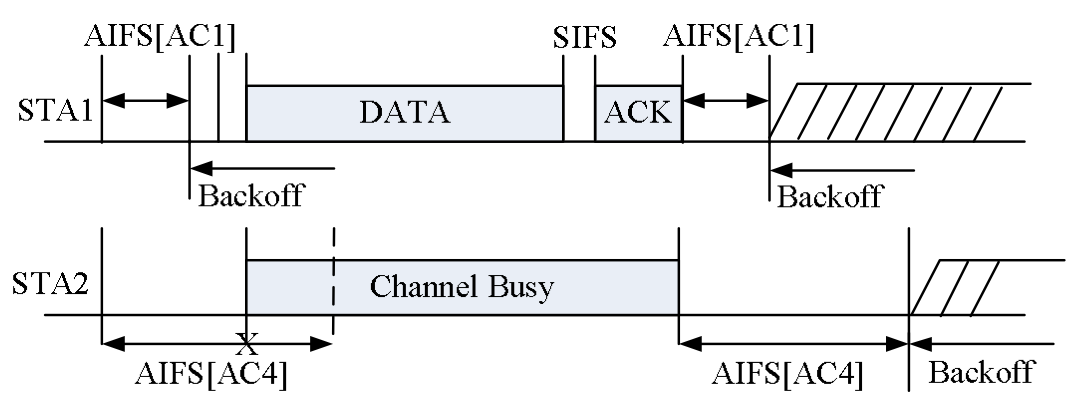
\includegraphics[width=0.7\textwidth]{aifs.png}
    \caption{Accesso al canale nell'EDCA}
    \label{fig:aifs}
\end{figure}

Ad ogni differente AC viene assegnata una differente coda; i vari frame vengono accodati nella coda appropriata in base alla \textit{Class Of Service (CoS)} di appartenenza; quest'ultime risultano essere quelle definite in un altro standard, ovvero l'IEEE 802.1D \cite{1309630}. Il mapping tra classe del frame e AC viene effettuata in questo modo (Tabella \ref{table:4}):

\begin{table}[h!]
    \centering
    \begin{tabular}{|>{\centering\arraybackslash}p{10em}|>{\centering\arraybackslash}p{7em}|} 
     \hline
     \textbf{AC} & \textbf{User Priorities} \\ 
     \hline
     \textbf{AC\_VO (Voice)} & 6, 7 \\ 
     \hline
     \textbf{AC\_VI (Video)} & 4, 5 \\
     \hline
     \textbf{AC\_BE (Best Effort)} & 0, 3 \\
     \hline
     \textbf{AC\_BK (Background)} & 1, 2 \\
     \hline
    \end{tabular}
    \caption{Mappature delle AC con le \textit{User Priorities}}
    \label{table:4}
\end{table}

E', comunque, sempre presente una sorta di casualità tra un AIFSN e un altro in modo da evitare che frame messi nella coda con priorità maggiore monopolizzino il canale a discapito di quelli a priorità minore.

\section{ITS-G5}
Dopo la definizione, da parte di IEEE, dello standard WAVE, in Europa si è reso necessario andare ad adattare i vari standard e normative allo scenario del vecchio continente.

\begin{figure}[h!]
    \centering
    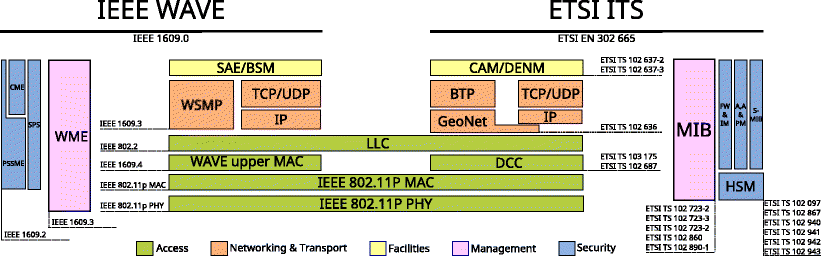
\includegraphics[width=1\textwidth]{wave_etsi.png}
    \caption{Parametri DCC con code EDCA}
    \label{fig:wave_etsi}
\end{figure}

Come è possibile notare dalla Figura \ref{fig:wave_etsi} \cite{etsi_security_standard}, i due standard condividono tutti i vari layer si occupano dell'accesso al canale, ovvero layer fisico, MAC e LLC, con la sola differenza che ITS prevede, in aggiunta, il \textit{Decentralized Congestion Control}, che verrà discusso in maniera approfondita nella \autoref{dcc}.

Qui una descrizione dei layer specifici di ITS, tralasciando quelli condivisi con WAVE in quanto se n'è già parlato precedentemente nella \autoref{wave}:

\begin{itemize}
    \item \textit{ETSI TS 102 636}: descrive le funzionalità per il \textit{GeoNetworking} \cite{etsi2013intelligent}; infatti anche qui è possibile utilizzare dei protocolli ad hoc anzichè TCP/UDP e IP, ovvero GeoNet e BTP (\textit{Basic Transport Protocol}) \cite{vogt2024comprehensive}.
    \item \textit{ETSI TS 723-x}: vari standard per definire le architetture e i requisiti per i sistemi di comunicazione DSRC \cite{etsi2012intelligent}.
    \item \textit{ETSI TS 102 943 e vari}: per tutto ciò che rigurda la sicurezza delle comunicazioni \cite{etsi2012intelligent_security}.
    \item \textit{ETSI TS 102 637-2/3}: messaggi CAM (\textit{Cooperative Awareness Message}) \cite{etsi2010102} e DENM (\textit{Decentralized Environmental Notification Message}) \cite{etsi2010etsi}.
\end{itemize}

Di tutto ciò, risultano di notevole importanza per questa trattazione i messaggi CAM e DENM e quindi richiedono un maggiore approfondimento.

\subsection[CAM]{CAM}
Il servizio CAM (Cooperative Awareness Message), definito dall'ETSI (European Telecommunications Standards Institute, 2011), fornisce una funzione di \textit{awareness} di base nelle reti ITS (Intelligent Transportation Systems) cooperative, attraverso l'invio periodico di dati di stato ai nodi adiacenti. Questo servizio funge da supporto per le applicazioni, consentendo la distribuzione regolare di messaggi contenenti informazioni sulla presenza, posizione e stato delle stazioni ITS.

I messaggi CAM vengono trasmessi alle stazioni ITS vicine che si trovano entro una distanza di un singolo hop dal mittente. Ricevendo questi messaggi, una stazione ITS può acquisire conoscenza delle altre stazioni nella sua area di prossimità, nonché delle loro posizioni, movimenti e caratteristiche rilevanti. Il destinatario di un messaggio CAM deve valutare la pertinenza delle informazioni ricevute, permettendo così alle stazioni ITS di ottenere dati utili sull'ambiente circostante e di reagire di conseguenza.

Lo standard ETSI definisce un insieme di informazioni che possono essere incluse in un messaggio CAM, rendendolo utile per varie applicazioni ITS, come l'avvicinamento di veicoli di emergenza o avvisi riguardanti veicoli lenti. Inoltre, lo standard è sufficientemente flessibile da permettere l'inclusione di nuove informazioni, garantendo la trasmissione di dati pertinenti per le applicazioni ITS \cite{cam_denm}.

Secondo la specifica ETSI TS 102 637-2 \cite{etsi2010102}, il formato di un messaggio CAM è composto da un \textit{header} e un \textit{body}. L'intestazione contiene informazioni sul messaggio stesso, come la versione, l'identificatore del messaggio e il tempo di generazione. Il corpo include dettagli sulla stazione ITS mittente, quali:

\begin{itemize}
    \item Identificatore univoco della stazione ITS.
    \item Tipo di stazione ITS (mobile, autorità pubblica, privata).
    \item Posizione di riferimento, espressa in termini di latitudine, longitudine, elevazione e direzione.
    \item Una serie di parametri CAM aggiuntivi, che possono essere inclusi facoltativamente in base al tipo di stazione ITS.
\end{itemize}

Oltre a specificare il formato dei messaggi CAM, lo standard ETSI fornisce anche indicazioni sui processi di gestione dei messaggi. Da un lato, vengono stabiliti requisiti temporali per la generazione periodica dei messaggi CAM, consentendo di regolare la frequenza in base al tipo di applicazione ITS per ottimizzare le prestazioni; è consentito l'invio ogni qualvolta il nodo presenta una variazione significativa delle sue coordinate spaziali, ovvero:

\begin{itemize}
    \item \textit{\textDelta \textalpha} maggiore di 4 gradi;
    \item \textDelta x maggiore di 5 metri;
    \item \textDelta v maggiore di 1 m/s;
\end{itemize}

Tali messaggi, tuttavia, non possono essere inviati con una frequenza superiore a 10 Hz e inferiore a 1 Hz.

Dall'altro lato, lo standard descrive le regole generali per la generazione dei messaggi, lasciando tuttavia agli sviluppatori delle applicazioni la libertà di prendere decisioni specifiche riguardo all'implementazione delle strutture CAM.

\subsection[DENM]{DENM}

\section[ETSI DCC]{Decentralized Congestion Control}
\label{dcc}
Le comunicazioni C-ITS devono funzionare anche in condizioni di traffico stradale intenso. Se tutti i veicoli partecipano allo scambio di informazioni C-ITS trasmettendo messaggi periodici, è probabile che si verifichi congestione nel canale wireless. Per evitare il degrado delle prestazioni del sistema causato da un carico eccessivo del canale e garantire un accesso equo alle risorse tra le stazioni ITS-G5 vicine (ITS-S), è necessario implementare meccanismi di controllo della congestione. A tal fine, l'ETSI ha pubblicato la specifica \textit{TS 102 687}, che definisce un meccanismo di controllo della congestione decentralizzato (\textit{DCC - Decentralized Congestion Control}) come parte dello stack di protocolli ITS-G5 \cite{8535090}. Il DCC è un componente obbligatorio dell'ITS-S e opera nella banda di frequenza dei 5,9 GHz.

Esso ha introdotto un approccio a macchina a stati finti al livello di accesso per adattare diversi parametri di trasmissione in base al carico del canale misurato. Ogni stato della macchina è associato a un determinato livello di carico del canale e a un insieme specifico di parametri di trasmissione. Questo consente al DCC di ottimizzare le comunicazioni in situazioni di congestione, migliorando l'efficienza e le prestazioni del sistema C-ITS.

Esistono diverse configurazioni che prevedono molteplici stati nella macchina di stato, ma verrà approfondita solo la configurazione \textit{DCC 2+1}, che comprende tre stati distinti: \textit{Relaxed}, \textit{Active} e \textit{Restrictive} (Figura \ref{fig:dcc}).

\begin{figure}[h!]
    \centering
    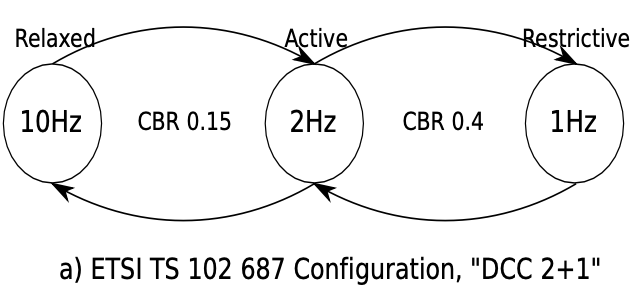
\includegraphics[width=0.7\textwidth]{dcc.png}
    \caption{DCC nella configurazione \textit{"2+1"}}
    \label{fig:dcc}
\end{figure}

In ciascuno stato del DCC vengono definite restrizioni sui parametri di trasmissione. L'ETSI DCC considera in generale cinque meccanismi per controllare l'accesso al canale del veicolo:

\begin{itemize}
    \item \textit{Transmit Power Control (TPC)} che adatta la potenza di trasmissione;
    \item \textit{Transmit Rate Control (TRC)} che adatta l'intervallo di trasmissione dei pacchetti;
    \item \textit{Transmit Datarate Control (TDC)} che adatta il \textit{data rate};
    \item \textit{DCC Sensitivity Control (DSC)} che adatta dinamicamente il \textit{CCA Sensitivity Threshold (CSThresh)}, ovvero la soglia sotto la quale il canale viene rilevato libero e non occupato;
    \item \textit{Transmit Access Control (TAC)} che apre e chiude dinamicamente l'accesso dei pacchetti con una determinata priorità alla relativa coda di trasmissione.
\end{itemize}

\noindent Maggiori dettagli su tali parametri verranno forniti nella \autoref{parametri_dcc}.

La scelta dello stato DCC si basa sulla valutazione del Channel Busy Ratio (CBR). L'ETSI propone un metodo di riferimento per stimare il valore del CBR consistente nel campionare tale valore ad intervalli prefissati per la durata di 1 secondo (Figura \ref{fig:cbr}); tale modello può, tuttavia, cambiare in base all'hardware utilizzato e al contesto di utilizzo.

\begin{figure}[h!]
    \centering
    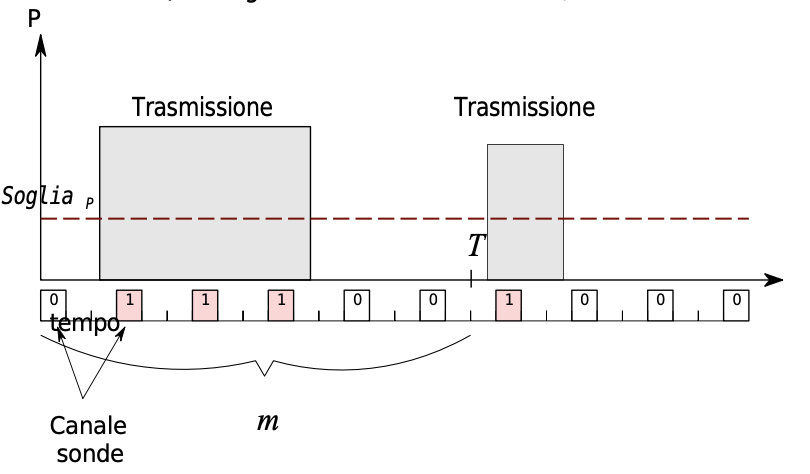
\includegraphics[width=0.7\textwidth]{cbr.png}
    \caption{Misurazione del CBR}
    \label{fig:cbr}
\end{figure}

Ogni transizione nella macchina a stati ha un valore CBR corrispondente come soglia (Figura \ref{fig:dcc}); la transizione viene eseguita in
una delle due condizioni seguenti:
\begin{itemize}
    \item \textit{Passaggio a uno stato più restrittivo}: se il valore CBR era superiore alla soglia durante l'ultimo intervallo di misurazione osservato.
    \item \textit{Passaggio a uno stato meno restrittivo}: se il CBR è stato inferiore alla soglia durante gli ultimi cinque intervalli di misurazione consecutivi osservati.
\end{itemize}

\subsection[Parametri DCC]{Parametri DCC}
\label{parametri_dcc}
Vengono mostrati i parametri relativi al DCC con i relativi valori in base allo stato \cite{6686471} (Tabella \ref{table:5}).

TPC (Transmit Power Control), DSC (DCC Sensitivity Control) e TRC (Transmit Rate Control) sono stati scelti per l'analisi perché sono direttamente rilevanti per le applicazioni di sicurezza cooperativa, dove la priorità è garantire comunicazioni affidabili e tempestive. Questi meccanismi si concentrano sull'ottimizzazione della potenza di trasmissione, della sensibilità e del tasso di trasmissione, elementi cruciali per mantenere la qualità del segnale e ridurre i ritardi in situazioni di congestione.

D'altra parte, TDC (Transmit Datarate Control) e TAC (Transmit Access Control) sono stati scartati per motivi specifici. La TDC è meno pertinente perché esiste un consenso consolidato nell'impostare a 6 Mbps la velocità di trasmissione per i messaggi di sicurezza, rendendo superflua la necessità di adattamenti dinamici della velocità. Questo approccio standardizzato garantisce una trasmissione stabile, essenziale in contesti critici.

La TAC, invece, è stata esclusa poiché si occupa principalmente della gestione della priorità tra diversi flussi di traffico, un aspetto meno rilevante per le comunicazioni di sicurezza. In questo contesto, l'obiettivo principale è garantire che i messaggi critici vengano trasmessi senza ritardi, piuttosto che gestire la priorità tra vari tipi di dati. Pertanto, concentrarsi su TPC, DSC e TRC consente di affrontare in modo più efficace le sfide specifiche delle comunicazioni di sicurezza cooperativa.

\begin{table}[h!]
    \centering
    \begin{tabular}{|>{\centering\arraybackslash}p{3em}|>{\centering\arraybackslash}p{5em}|>{\centering\arraybackslash}p{7em}|>{\centering\arraybackslash}p{7em}|>{\centering\arraybackslash}p{7em}|} 
     \hline
     \textbf{Scheme} & \textbf{Metric} & \textbf{RELAXED} & \textbf{ACTIVE} & \textbf{RESTRICTIVE} \\ 
     \hline
     \textbf{TPC} & \textit{\( P_{t} \)} & 35 dBm & 15 dBm & -10 dBm \\ 
     \hline
     \textbf{DSC} & \textit{CSThresh} & -95 dBm & -85 dBm & -65 dBm \\
     \hline
     \textbf{TRC} & Pack. inter. & 0.04 s & 0.5 s & 1 s\\
     \hline
    \end{tabular}
    \caption{Parametri DCC}
    \label{table:5}
\end{table}

Degno di nota il fatto che, nonostante i validi obiettivi delle tecniche DCC specificate dall'ETSI, finora solo pochi studi hanno analizzato le loro prestazioni. Ci sono solo alcuni lavori, come quello di Subramanian et al. \cite{subramanian2012congestion}, ove tutti i meccanismi DCC sono stati attivati in modo simulato, e i risultati indicano che non sono efficaci nel controllare la congestione e garantire la raggiungibilità. Gli autori propongono quindi miglioramenti alla tecnica TPC, progettando una macchina a stati con sei stati e una soglia di carico del canale più alta per lo stato di congestione. Tuttavia, entrambi i lavori non distinguono gli effetti di ciascun meccanismo.

\subsection[DCC con code EDCA]{Parametri DCC con code EDCA}

In aggiunta alle tecniche di controllo della congestione già specificate, l'ETSI ha introdotto parametri aggiuntivi in base alle categorie di accesso (Access Categories, AC) utilizzate \cite{etsi2011intelligent} (Figura \ref{fig:dcc_edca}). Queste categorie sono fondamentali per gestire le diverse priorità e requisiti di latenza delle comunicazioni veicolari. Ogni Access Category è associata a specifiche caratteristiche di traffico, consentendo una gestione più fine delle risorse di comunicazione.

Ad esempio, le applicazioni critiche per la sicurezza, come i messaggi di avviso e le comunicazioni di emergenza, possono essere classificate in una categoria di accesso con priorità più alta. Ciò implica l'adozione di parametri di controllo della congestione più stringenti per garantire che questi messaggi vengano trasmessi senza ritardi. Al contrario, le comunicazioni meno critiche possono essere assegnate a categorie con requisiti di latenza e affidabilità inferiori, permettendo una gestione più flessibile delle risorse di rete.

Questa suddivisione in Access Categories consente all'ETSI di ottimizzare le prestazioni del sistema, migliorando l'efficacia delle tecniche di controllo della congestione e garantendo che le comunicazioni più importanti ricevano la priorità necessaria in situazioni di traffico intenso.

\begin{figure}[h!]
    \centering
    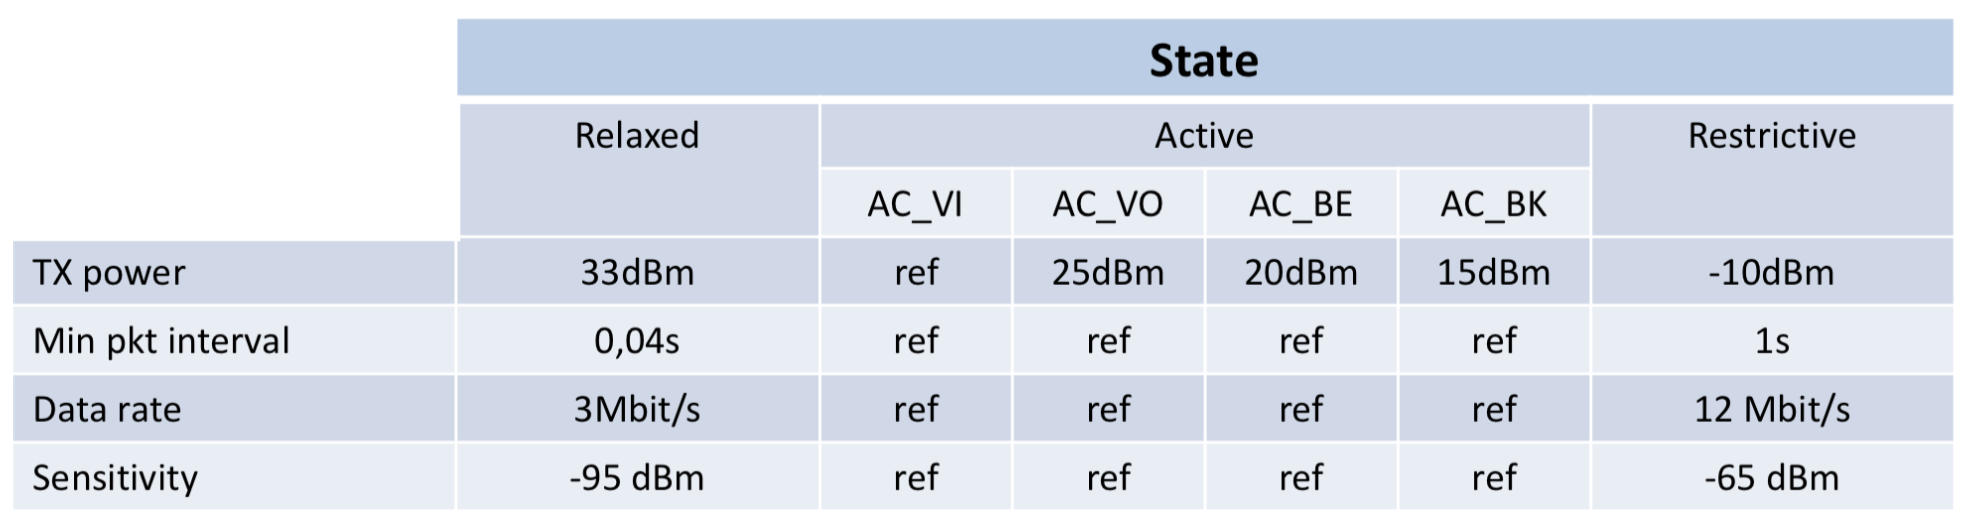
\includegraphics[width=1\textwidth]{dcc_edca.png}
    \caption{Parametri DCC con code EDCA}
    \label{fig:dcc_edca}
\end{figure}

Il valore \textit{ref} indica che il parametro è invariato e viene utilizzato il valore precedente del parametro di riferimento corrispondente.

Da come si può notare in figura \ref{fig:dcc_edca}, in questo contesto non è stata esclusa la \textit{Transmit Datarate Control}, in quanto, vista l'applicazione del DCC con code EDCA in contesti generici e non strettamente legati alla sicurezza, non aveva più senso basarsi sullo standard \textit{de facto} della velocità di trasmissione di 6 Mbps.
